% Options for packages loaded elsewhere
% Options for packages loaded elsewhere
\PassOptionsToPackage{unicode}{hyperref}
\PassOptionsToPackage{hyphens}{url}
\PassOptionsToPackage{dvipsnames,svgnames,x11names}{xcolor}
%
\documentclass[
  letterpaper,
  DIV=11,
  numbers=noendperiod]{scrreprt}
\usepackage{xcolor}
\usepackage{amsmath,amssymb}
\setcounter{secnumdepth}{5}
\usepackage{iftex}
\ifPDFTeX
  \usepackage[T1]{fontenc}
  \usepackage[utf8]{inputenc}
  \usepackage{textcomp} % provide euro and other symbols
\else % if luatex or xetex
  \usepackage{unicode-math} % this also loads fontspec
  \defaultfontfeatures{Scale=MatchLowercase}
  \defaultfontfeatures[\rmfamily]{Ligatures=TeX,Scale=1}
\fi
\usepackage{lmodern}
\ifPDFTeX\else
  % xetex/luatex font selection
\fi
% Use upquote if available, for straight quotes in verbatim environments
\IfFileExists{upquote.sty}{\usepackage{upquote}}{}
\IfFileExists{microtype.sty}{% use microtype if available
  \usepackage[]{microtype}
  \UseMicrotypeSet[protrusion]{basicmath} % disable protrusion for tt fonts
}{}
\makeatletter
\@ifundefined{KOMAClassName}{% if non-KOMA class
  \IfFileExists{parskip.sty}{%
    \usepackage{parskip}
  }{% else
    \setlength{\parindent}{0pt}
    \setlength{\parskip}{6pt plus 2pt minus 1pt}}
}{% if KOMA class
  \KOMAoptions{parskip=half}}
\makeatother
% Make \paragraph and \subparagraph free-standing
\makeatletter
\ifx\paragraph\undefined\else
  \let\oldparagraph\paragraph
  \renewcommand{\paragraph}{
    \@ifstar
      \xxxParagraphStar
      \xxxParagraphNoStar
  }
  \newcommand{\xxxParagraphStar}[1]{\oldparagraph*{#1}\mbox{}}
  \newcommand{\xxxParagraphNoStar}[1]{\oldparagraph{#1}\mbox{}}
\fi
\ifx\subparagraph\undefined\else
  \let\oldsubparagraph\subparagraph
  \renewcommand{\subparagraph}{
    \@ifstar
      \xxxSubParagraphStar
      \xxxSubParagraphNoStar
  }
  \newcommand{\xxxSubParagraphStar}[1]{\oldsubparagraph*{#1}\mbox{}}
  \newcommand{\xxxSubParagraphNoStar}[1]{\oldsubparagraph{#1}\mbox{}}
\fi
\makeatother


\usepackage{longtable,booktabs,array}
\usepackage{calc} % for calculating minipage widths
% Correct order of tables after \paragraph or \subparagraph
\usepackage{etoolbox}
\makeatletter
\patchcmd\longtable{\par}{\if@noskipsec\mbox{}\fi\par}{}{}
\makeatother
% Allow footnotes in longtable head/foot
\IfFileExists{footnotehyper.sty}{\usepackage{footnotehyper}}{\usepackage{footnote}}
\makesavenoteenv{longtable}
\usepackage{graphicx}
\makeatletter
\newsavebox\pandoc@box
\newcommand*\pandocbounded[1]{% scales image to fit in text height/width
  \sbox\pandoc@box{#1}%
  \Gscale@div\@tempa{\textheight}{\dimexpr\ht\pandoc@box+\dp\pandoc@box\relax}%
  \Gscale@div\@tempb{\linewidth}{\wd\pandoc@box}%
  \ifdim\@tempb\p@<\@tempa\p@\let\@tempa\@tempb\fi% select the smaller of both
  \ifdim\@tempa\p@<\p@\scalebox{\@tempa}{\usebox\pandoc@box}%
  \else\usebox{\pandoc@box}%
  \fi%
}
% Set default figure placement to htbp
\def\fps@figure{htbp}
\makeatother





\setlength{\emergencystretch}{3em} % prevent overfull lines

\providecommand{\tightlist}{%
  \setlength{\itemsep}{0pt}\setlength{\parskip}{0pt}}



 


\KOMAoption{captions}{tableheading}
\makeatletter
\@ifpackageloaded{bookmark}{}{\usepackage{bookmark}}
\makeatother
\makeatletter
\@ifpackageloaded{caption}{}{\usepackage{caption}}
\AtBeginDocument{%
\ifdefined\contentsname
  \renewcommand*\contentsname{Table of contents}
\else
  \newcommand\contentsname{Table of contents}
\fi
\ifdefined\listfigurename
  \renewcommand*\listfigurename{List of Figures}
\else
  \newcommand\listfigurename{List of Figures}
\fi
\ifdefined\listtablename
  \renewcommand*\listtablename{List of Tables}
\else
  \newcommand\listtablename{List of Tables}
\fi
\ifdefined\figurename
  \renewcommand*\figurename{Figure}
\else
  \newcommand\figurename{Figure}
\fi
\ifdefined\tablename
  \renewcommand*\tablename{Table}
\else
  \newcommand\tablename{Table}
\fi
}
\@ifpackageloaded{float}{}{\usepackage{float}}
\floatstyle{ruled}
\@ifundefined{c@chapter}{\newfloat{codelisting}{h}{lop}}{\newfloat{codelisting}{h}{lop}[chapter]}
\floatname{codelisting}{Listing}
\newcommand*\listoflistings{\listof{codelisting}{List of Listings}}
\makeatother
\makeatletter
\makeatother
\makeatletter
\@ifpackageloaded{caption}{}{\usepackage{caption}}
\@ifpackageloaded{subcaption}{}{\usepackage{subcaption}}
\makeatother
\usepackage{bookmark}
\IfFileExists{xurl.sty}{\usepackage{xurl}}{} % add URL line breaks if available
\urlstyle{same}
\hypersetup{
  pdftitle={Armein Z. R. Langi},
  pdfauthor={131902360 Armein Z R Langi},
  colorlinks=true,
  linkcolor={blue},
  filecolor={Maroon},
  citecolor={Blue},
  urlcolor={Blue},
  pdfcreator={LaTeX via pandoc}}


\title{Armein Z. R. Langi}
\usepackage{etoolbox}
\makeatletter
\providecommand{\subtitle}[1]{% add subtitle to \maketitle
  \apptocmd{\@title}{\par {\large #1 \par}}{}{}
}
\makeatother
\subtitle{Portfolio Asesmen II-2100 KIPP}
\author{131902360 Armein Z R Langi}
\date{2025-09-15}
\begin{document}
\maketitle

\renewcommand*\contentsname{Table of contents}
{
\hypersetup{linkcolor=}
\setcounter{tocdepth}{2}
\tableofcontents
}

\bookmarksetup{startatroot}

\chapter*{Selamat Berjumpa}\label{selamat-berjumpa}
\addcontentsline{toc}{chapter}{Selamat Berjumpa}

\markboth{Selamat Berjumpa}{Selamat Berjumpa}

\begin{figure}[H]

{\centering \includegraphics[width=9.5\linewidth,height=\textheight,keepaspectratio]{images/AZRL.png}

}

\caption{About Me}

\end{figure}%

Rezky Muhammad Hafiz Batubara adalah mahasiswa angkatan 2024 di jurusan
Sistem dan Teknologi Informasi di Sekolah Teknik Elektro dan Informatika
ITB, mahasiswa sejak Juli 2024, bersekolah SMA di SMA Labschool Cibubur.

Lahir di Jakarta 22 November 2006. Saat ini tinggal di Bandung, di Dago
Asri.

Kontak LinkedIn ada di
https://www.linkedin.com/in/rezky-muhammad-hafiz-batubara-606b73337/.

\bookmarksetup{startatroot}

\chapter{UTS-1 All About Me}\label{uts-1-all-about-me}

\begin{figure}[H]

{\centering 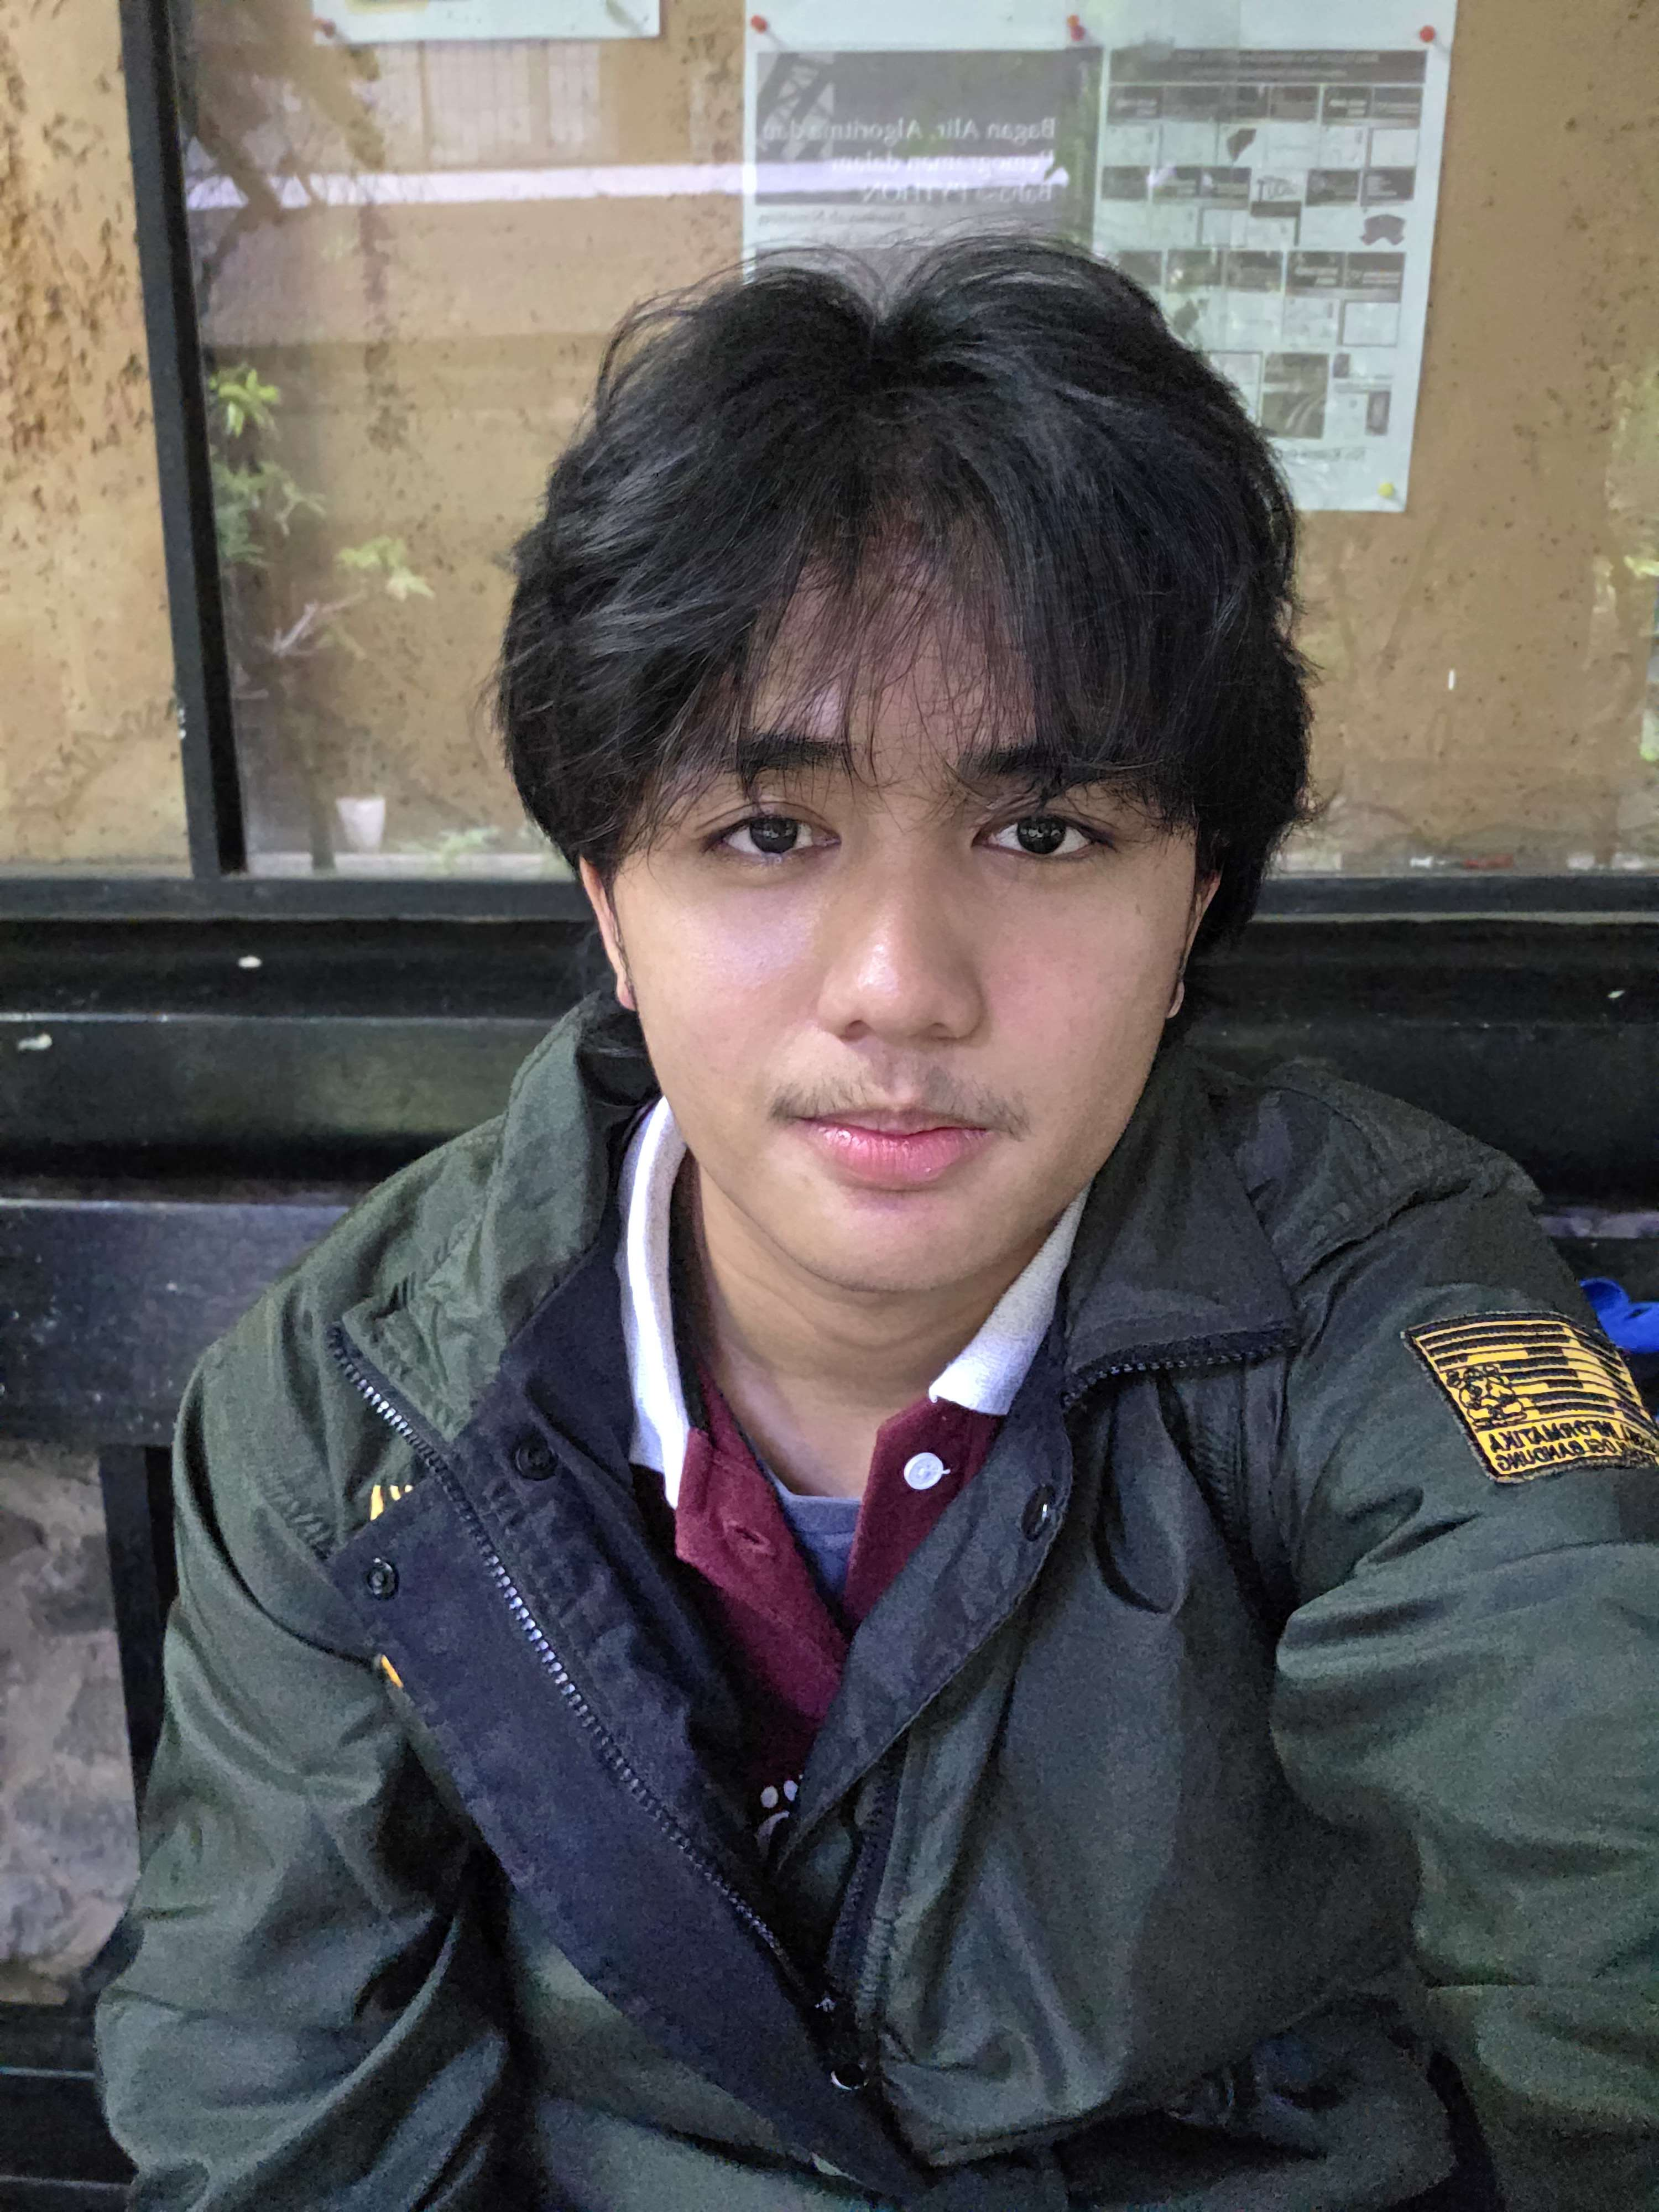
\includegraphics[width=9.5\linewidth,height=\textheight,keepaspectratio]{All_About_me/../images/RezkyHMIF_KIPP.jpg}

}

\caption{About Me}

\end{figure}%

Halo, namaku Rezky Muhammad Hafiz Batubara dengan panggilan rezky atau
ky. Aku adalah mahasiswa angkatan 2024 di jurusan Sistem dan Teknologi
Informasi di Sekolah Teknik Elektro dan Informatika ITB. Aku seorang
mahasiswa yang selalu percaya bahwa belajar bukan hanya soal menambah
pengetahuan, tetapi juga tentang memahami diri sendiri dan menikmati
setiap prosesnya. Aku suka belajar, tapi aku juga percaya bahwa hidup
tidak bisa diisi dengan keseriusan terus-menerus. Kadang, cara terbaik
untuk memahami sesuatu justru datang saat kita memberi ruang untuk
bersenang-senang, entah dengan menikmati waktu sendiri, atau berbagi
tawa dengan orang lain.

Sejak kecil, rasa ingin tahuku sudah seperti refleks alami. Aku selalu
penasaran terhadap hal-hal yang belum kupahami. Saat SD, aku pernah ikut
lomba Matematika Nalar, dan di sanalah untuk pertama kalinya aku belajar
tentang arti kompetisi. Aku sadar bahwa berkompetisi bukan soal
mengalahkan orang lain, tapi tentang bagaimana menantang diri sendiri
untuk berpikir lebih dalam dan lebih tenang di bawah tekanan.

Saat SMA, aku mulai memahami arti kerja keras sesungguhnya. Aku belajar
dengan sungguh-sungguh, sering kali larut malam, bukan karena ingin
terlihat pintar, tapi karena aku tahu setiap usaha akan membawa aku
lebih dekat pada versi terbaik dari diriku sendiri. Sekarang, di dunia
perkuliahan, rasa ingin tahu itu tidak pernah hilang, hanya berubah
bentuk. Aku mulai tertarik dengan dunia data dan mencoba memahami
bagaimana angka dan informasi bisa bercerita. Aku ikut beberapa lomba
dan tantangan belajar, bukan semata-mata untuk menang, tetapi karena aku
ingin terus mengasah logika dan menumbuhkan cara berpikir yang lebih
kritis.

Namun, di balik semangat belajar itu, aku juga tahu kapan harus berhenti
sejenak. Aku suka menghabiskan waktu sendiri baik dengan bermain game,
menonton film, atau sekedar duduk sambil memikirkan beberapa hal. Selain
itu, aku juga senang menghabiskan waktu dengan teman-teman, tertawa,
berdiskusi, atau membicarakan hal-hal ringan yang sering kali justru
memberi inspirasi baru. Dari situ aku belajar, \textbf{keseimbangan
adalah bagian penting dari pertumbuhan.} Belajar tanpa jeda membuat
pikiran kaku; bersenang-senang tanpa arah membuat langkah kehilangan
makna.

Aku pernah membaca kalimat, \emph{``Curiosity makes you grow, but
balance keeps you alive.''} Dan aku sangat percaya pada itu. Karena bagi
saya, belajar bukan hanya soal menambah ilmu, tapi tentang membangun
kebijaksanaan, tentang kapan harus berjuang, kapan harus berhenti
sejenak, dan kapan harus tertawa.

Kini, setiap kali aku menatap layar dan mencoba memahami hal baru, aku
tahu satu hal: perjalanan ini bukan tentang menjadi yang paling tahu,
tapi tentang menjadi orang yang tidak berhenti belajar. Karena dunia
selalu berubah, dan aku ingin menjadi bagian dari perubahan itu, bukan
hanya dengan berpikir, tetapi juga dengan menikmati setiap langkahnya.

\begin{center}\rule{0.5\linewidth}{0.5pt}\end{center}

\section{1.1 Kisah yang Membentuk Diri Anda: Mengenal Kekuatan Identitas
Naratif}\label{kisah-yang-membentuk-diri-anda-mengenal-kekuatan-identitas-naratif}

Setiap orang punya kisah yang membentuk cara mereka memandang dunia.
Bagiku, kisah itu dimulai dari rasa ingin tahu yang sederhana, tentang
mengapa sesuatu bekerja seperti itu, bagaimana data bisa menjelaskan
fenomena, atau mengapa sebuah masalah bisa punya banyak jalan keluar.

Namun, kekuatanku bukan hanya terletak pada rasa ingin tahu itu,
melainkan pada kemampuanku untuk \textbf{menikmati proses belajar}. Aku
menyadari bahwa perjalanan memahami dunia bukanlah lomba cepat, tapi
maraton panjang. Di sinilah aku belajar bahwa identitas naratifku
terbentuk dari \textbf{keseimbangan antara berpikir dan beristirahat,
antara bekerja keras dan menikmati waktu bersama orang-orang yang
kusayangi.}

\begin{center}\rule{0.5\linewidth}{0.5pt}\end{center}

\section{1.1.1 Tiga Lapisan Diri Anda: Di Mana Cerita Hidup Anda
Berada?}\label{tiga-lapisan-diri-anda-di-mana-cerita-hidup-anda-berada}

\textbf{Level 1 -- Sifat Dasar:}\\
Aku adalah orang yang tenang, analitis, dan reflektif. Aku suka berpikir
dalam-dalam tentang sesuatu, tapi juga tahu kapan harus berhenti untuk
tertawa.

\textbf{Level 2 -- Kepedulian Pribadi:}\\
Aku menjunjung tinggi kerja keras, rasa ingin tahu, dan keseimbangan.
Aku percaya bahwa kemampuan bernalar dan belajar adalah kekuatan
terbesar manusia, tetapi kemampuan untuk menikmati proses adalah yang
membuat kita tetap waras dan bahagia.

\textbf{Level 3 -- Identitas Naratif:}\\
Cerita hidupku adalah kisah tentang seseorang yang mencintai proses
belajar, tapi juga menghargai waktu untuk bersenang-senang. Aku percaya
bahwa pertumbuhan terbaik muncul ketika pikiran tajam dan hati tetap
ringan.

\begin{center}\rule{0.5\linewidth}{0.5pt}\end{center}

\section{1.1.2 Pola-Pola Kisah Kehidupan: Apa yang Membuat Sebuah Cerita
Bermanfaat?}\label{pola-pola-kisah-kehidupan-apa-yang-membuat-sebuah-cerita-bermanfaat}

Jika kulihat ke belakang, pola hidupku adalah \textbf{pola pembelajaran
yang lentur}, bagaimana aku belajar dari kesalahan tanpa menjadikannya
beban, dan bagaimana aku mencari makna di balik hal-hal kecil.

Kisah hidup menjadi bermanfaat ketika ia \textbf{menginspirasi orang
lain untuk terus bertumbuh tanpa kehilangan sisi manusianya.} Aku
belajar bahwa berbagi semangat belajar dan rasa ingin tahu bukan berarti
harus terlihat sempurna, tetapi tentang menunjukkan bahwa proses yang
jujur pun bisa menjadi sumber inspirasi.

\begin{center}\rule{0.5\linewidth}{0.5pt}\end{center}

\section{1.1.3 Seni Memberi Makna: Kekuatan Super Anda dalam
Bernalar}\label{seni-memberi-makna-kekuatan-super-anda-dalam-bernalar}

Jika aku punya kekuatan super, itu adalah kemampuan \textbf{bernalar
dengan tenang di tengah kerumitan.} Aku senang menelusuri sebab-akibat,
mencari pola di balik data, atau sekadar memahami alasan di balik suatu
peristiwa.

Namun kekuatan itu tidak hanya bekerja dalam logika, tetapi juga dalam
kehidupan. Bernalar membuatku mampu memahami bahwa tidak semua hal bisa
diselesaikan cepat, kadang yang kita butuhkan hanyalah waktu, kesabaran,
dan sedikit humor untuk melihat situasi dari sudut lain.

Bagi diriku, bernalar bukan hanya alat untuk berpikir, tapi juga
\textbf{cara untuk memberi makna.} Ia mengubah rasa frustrasi menjadi
rasa ingin tahu baru, dan mengubah kebingungan menjadi dorongan untuk
terus belajar.

\begin{center}\rule{0.5\linewidth}{0.5pt}\end{center}

\section{1.1.4 Mulai Menulis Ulang Kisah Anda: Dua Langkah
Praktis}\label{mulai-menulis-ulang-kisah-anda-dua-langkah-praktis}

\textbf{Langkah pertama:}\\
Terima bahwa belajar tidak harus selalu serius. Dulu aku sering berpikir
bahwa menjadi ``pintar'' berarti harus selalu fokus dan efisien. Tapi
ternyata, memberi ruang untuk bersenang-senang justru membuat pikiranku
lebih jernih dan ide-ide baru muncul lebih alami.

\textbf{Langkah kedua:}\\
Tulis ulang cara pandang terhadap kegagalan. Aku tidak lagi melihat
kesalahan sebagai tanda kelemahan, tapi sebagai bahan bakar rasa ingin
tahu. Saat sebuah ide tidak berjalan, aku belajar menertawakannya,
merenungkannya, lalu mencoba lagi dengan cara berbeda.

Dengan dua langkah sederhana ini, aku menemukan kedamaian dalam proses
belajar: bahwa gagal pun bisa terasa menyenangkan jika kita tahu cara
menikmatinya.

\begin{center}\rule{0.5\linewidth}{0.5pt}\end{center}

\section{1.1.5 Kesimpulan: Kisah Anda Adalah Perjalanan yang Terus
Berlanjut}\label{kesimpulan-kisah-anda-adalah-perjalanan-yang-terus-berlanjut}

Kini aku menyadari bahwa kisah hidupku bukan tentang pencapaian, tapi
tentang perjalanan yang tidak pernah selesai. Dari lomba matematika di
masa kecil hingga belajar memahami pola data hari ini, semua adalah
bab-bab yang saling terhubung.

Aku ingin terus menulis kisah ini, dengan \textbf{rasa ingin tahu yang
sama, semangat belajar yang sama, dan tawa yang menyeimbangkan
semuanya.} Karena bagi aku, hidup yang baik bukan hanya tentang menjadi
lebih pintar, tapi juga tentang menjadi lebih bijak, lebih tenang, dan
lebih bahagia di setiap langkahnya.

\bookmarksetup{startatroot}

\chapter{UTS-2 My Songs for You}\label{uts-2-my-songs-for-you}

Post Wedding Kawah Putih Lirik by Armein Z. R. Langi Music: SUNO

\url{https://youtu.be/KWthEImJ9mY?si=iUV8Ghhj0R3gKQyZ}

Why am I singing for you? \href{./Rivers\%20In\%20My\%20Mind.mp3}{River
in my Mind}

Falling in love everyday \href{./Heaven\%20on\%20Earth.mp3}{Heaven on
Earth}

\bookmarksetup{startatroot}

\chapter{UTS-3 My Stories for You}\label{uts-3-my-stories-for-you}

A story about my oldest daughter
\href{https://azrl.wordpress.com/2020/07/18/gaun-pengantin-gladys/\#comment-28004}{Gaun
Pemngantin Gladys}

A message to my daughter
\href{https://azrl.wordpress.com/2021/10/06/the-child-who-learned-to-walk-at-the-disneyland/}{The
Child Who Learned to Walk at the Disneyland}

A story for my students
\href{https://azrl.wordpress.com/2008/04/21/fly-my-eagle-fly/}{Fly Eagle
Fly}

A (true) story for my teachers
\href{\%3Chttps://azrl.wordpress.com/2012/11/28/perginya-sang-mahaputera-dan-mahaguru-berkemeja-putih/}{Sang
Mahaguru, Sang Mahaputera}

Teasing story \url{https://www.youtube.com/watch?v=Dg_4PbBlBf4}

\bookmarksetup{startatroot}

\chapter{UTS-5 My Shapes}\label{uts-5-my-shapes}

\bookmarksetup{startatroot}

\chapter{My Personal Reviews}\label{my-personal-reviews}

Berikut cara saya melakukan review
\href{./Doc.5.Mengevaluasi-Esai-Berdasarkan-Rubrik.pdf}{Menilai dan
Mengevaluasi Esai Berdasarkan Rubrik}

\bookmarksetup{startatroot}

\chapter{UAS-1 My Concepts}\label{uas-1-my-concepts}

Mau hidup epik ? \href{lifestory.pdf}{Write your Life Story}

Apa itu berkonsep?

\url{https://youtu.be/QVfUlVBO80U?si=yM6q_rwV9rcDBbu7}

\bookmarksetup{startatroot}

\chapter{UAS-3 My Opinions}\label{uas-3-my-opinions}

SApa itu beropini? \href{BM\%20Opini.mp4}{Opini Berpengaruh}

Bagiamana menjaadi menarik? \href{./Interesting.mp4}{Menjadi Menarik}

\bookmarksetup{startatroot}

\chapter{UAS-3 My Innovations}\label{uas-3-my-innovations}

\bookmarksetup{startatroot}

\chapter{UAS-4 My Knowledge}\label{uas-4-my-knowledge}

Cara saya mengkomunikasikan sebuah pengatahuan sebagai petunjuk bagi
orang lain 1) saya tulis
\href{Rekomendasi\%20Presentasi\%20Efektif(Contoh\%20Makalah).pdf}{makalah
sebagai bahan utama} 2) lalu saya buat
\href{Contoh\%20Transkrip\%20Presentasi.pdf}{transkrip ucapan lisan} 3)
kemudian saya kembangkan
\href{Rekomendasi\%20Presentasi\%20(Contoh\%20Slides).pdf}{slide
pendukung trnsskrip} 4) lalu saya memproduksivideo audio visual
\url{https://youtu.be/ZbghfMvnPZc} \url{https://youtu.be/ZbghfMvnPZc}

\bookmarksetup{startatroot}

\chapter{UAS-5 My Professional
Reviews}\label{uas-5-my-professional-reviews}

Untuk melAkukan review, seperti pada
\href{../My_Personal_Reviews/Doc.5.Mengevaluasi-Esai-Berdasarkan-Rubrik.pdf}{pendekatan
AI}, kita membutuhkan rubrik

\bookmarksetup{startatroot}

\chapter{Summary}\label{summary}

In summary, this book has no content whatsoever.

\bookmarksetup{startatroot}

\chapter*{References}\label{references}
\addcontentsline{toc}{chapter}{References}

\markboth{References}{References}

\phantomsection\label{refs}




\end{document}
